\documentclass[tikz,border=8pt]{standalone}
\usepackage{ctex}
\usepackage{amsmath,amssymb,bm}
\usetikzlibrary{arrows.meta,calc,angles,quotes,decorations.pathmorphing,patterns,positioning,3d,circuits.ee.IEC}
\definecolor{ink}{RGB}{30,43,58}
\definecolor{blue}{RGB}{37,91,166}
\definecolor{orange}{RGB}{219,113,25}
\definecolor{green}{RGB}{39,139,94}
\definecolor{red}{RGB}{192,52,52}
\tikzset{
 line cap=round,line join=round,
 body/.style={draw=ink,very thick},
 axis/.style={-{Latex[length=2.5mm]},draw=ink,very thick},
 vec/.style={-{Latex[length=2.5mm]},draw=blue,very thick},
 force/.style={-{Latex[length=2.5mm]},draw=red,very thick},
 guide/.style={draw=ink!45,dashed},
 dim/.style={{Latex[length=2mm]}-{Latex[length=2mm]},draw=ink!75},
 current/.style={-{Latex[length=2.5mm]},draw=orange,very thick}
}

\tikzset{mass/.style={circle,draw,fill=white,minimum size=7mm},curve/.style={very thick,blue},rope/.style={very thick,blue},ray/.style={very thick,blue,-{Latex}},impulse/.style={very thick,orange,-{Latex}},resistor/.style={thick,decorate,decoration={zigzag,segment length=3mm,amplitude=1mm}}}
\begin{document}
% 1 question-01
\begin{tikzpicture}[scale=1]
  \draw[axis] (-1.4,0)--(5.6,0) node[right] {$x$};
  \draw[axis] (0,-3.1)--(0,3.2) node[above] {$y$};
  \filldraw[fill=white,body] (3.5,0) circle(4pt) node[below=5pt] {蔡子星};
  \filldraw[fill=white,body] (0,0) circle(4pt) node[above left] {黄伯星};
  \draw[dim] (0,.65)--(3.5,.65) node[midway,above] {$L$};
  \draw[vec] (0,-.15)--(0,-1.65) node[left] {$u_0$};
  \coordinate (C) at (1.75,0);
  \fill[orange] (C) circle(3pt) node[above right] {中点星人};
  \node[align=center] at (2.3,-2.7) {两星球分别沿坐标轴运动，中点始终位于连线中点};
\end{tikzpicture}

% 2 solution-01
\begin{tikzpicture}[x=1cm,y=1cm,font=\small]

\draw[axis](-2.1,0)--(4.7,0)node[right]{$X$};\draw[axis](0,-2.9)--(0,2.9)node[above]{$Y$};
\draw[body,blue](1,0)ellipse(2.5 and 2.291288);\fill(0,0)circle(2pt)node[below left]{$O$（焦点）};\fill(1,0)circle(2pt)node[above]{$C$（中心）};
\fill(3.5,0)circle(2pt)node[above right]{$L/2$};\draw[vec](3.5,0)--(3.5,-1.2)node[right]{$u_0/2$};\draw[dim](-1.5,-2.7)--(3.5,-2.7)node[midway,below]{$2a$};
\node[align=left,anchor=west]at(5.8,0){示例$u_0^2=0.6Gm/L$\\$a=5L/14,c=L/7$\\$M_{\rm eff}=m/8$};
\end{tikzpicture}

% 3 question-02
\begin{tikzpicture}[scale=.9]
  % 水平圆盘及其竖直转轴。
  \coordinate (O) at (1.1,-1.45);
  \fill[blue!9] (O) ellipse (4.1 and 1.18);
  \draw[body] (O) ellipse (4.1 and 1.18);
  \draw[guide] (1.1,-3.1)--(1.1,2.3) node[above] {竖直转轴};
  \fill (O) circle(2pt) node[below right] {$O$};
  \draw[dim] (1.1,-2.85)--(5.2,-2.85) node[midway,below] {$R$};

  % A 在圆盘轴线上且高出盘面 r；滚筒中心轴 AA' 向左延伸。
  \coordinate (A) at (1.1,.05);
  \coordinate (Aprime) at (-4.7,.05);
  \draw[guide] (A)--(Aprime);
  \draw[body,fill=orange!18]
    (Aprime) ++(0,-.62) -- ($(A)+(0,-.62)$)
    arc[start angle=-90,end angle=90,x radius=.28,y radius=.62]
    -- ($(Aprime)+(0,.62)$)
    arc[start angle=90,end angle=270,x radius=.28,y radius=.62] -- cycle;
  \draw[body] (A) ellipse (.28 and .62);
  \draw[body] (Aprime) ellipse (.28 and .62);
  \fill (A) circle(2.4pt) node[above right] {$A$};
  % A' 端在竖直光滑限位器内滑动。
  \fill[ink!6] (-5.35,-1.65)--(-4.92,-1.45)--(-4.92,2.05)--(-5.35,2.25)--cycle;
  \draw[body] (-5.35,-1.65)--(-5.35,2.25)--(-4.92,2.05)--(-4.92,-1.45)--cycle;
  \draw[body] (-4.7,-1.05)--(-4.7,1.15);
  \node[below right] at (-4.62,-.7) {$A'$};
  \node[anchor=south] at (-5.15,2.28) {限位器};

  \draw[dim] ($(Aprime)+(0,1.05)$)--($(A)+(0,1.05)$)
    node[midway,above] {$mR$};
  \draw[dim] ($(A)+(.65,-1.45)$)--($(A)+(.65,0)$)
    node[midway,right] {$r=nR$};
  \draw[current] (-3.9,.85) arc[start angle=140,end angle=430,x radius=.75,y radius=.35]
    node[above left] {$\omega_0$};
  \node at (0,-3.65) {圆盘绕竖直轴转动；滚筒中心轴为 $AA'$};
\end{tikzpicture}

% 4 solution-02
\begin{tikzpicture}[x=1cm,y=1cm,font=\small]

\draw[body,fill=blue!5](0,0)circle(3);\draw[very thick,orange](0,0)--(3,0);\node[orange]at(1.2,-.7){径向接触线};
\fill(0,0)circle(2pt)node[below left]{$O$};
\fill (2.381102,0.000000) circle(2pt) node[below] {$\lambda R$};

\draw[force](1,0)--(1,1.1)node[left]{驱动};\draw[force](2.7,0)--(2.7,-1.1)node[right]{制动};
\node[align=left,anchor=west]at(4.5,.5){$\lambda=2^{-1/3}$\\$\omega_1\lambda R=\omega_0nR$\\$\int_0^\lambda\rho^2\mathrm d\rho=\int_\lambda^1\rho^2\mathrm d\rho$};\node at(0,-3.7){只有接触线上的一个点无相对滑动};
\end{tikzpicture}

% 5 question-03
\begin{tikzpicture}[x=1cm,y=1cm,font=\small]

\draw[body,fill=blue!7](0,0)circle(1.6);\fill(0,0)circle(2pt)node[below right]{轴};\draw[dim](0,.2)--(1.6,.2)node[midway,above]{$R$};
\draw[body](-1.6,0)--(-1.6,-3.7);\node[mass]at(-1.6,-3.9){$m$};\node[draw,circle,dashed]at(-1.6,-2.5){$m$};\draw[dim](-2.3,-2.5)--(-2.3,-3.9)node[midway,left]{$H$};
\draw[force](-1.6,-3.9)--(-1.6,-5)node[right]{$mg$};\draw[impulse](1.1,1.1)arc(45:130:1.556)node[above]{$\omega,\beta$};
\node at(0,2.4){端面：轻绳沿左外缘相切};
\begin{scope}[shift={(4.8,0)}]\draw[body,fill=blue!7](-1.7,-.6)rectangle(1.7,.6);\draw[dim](-1.7,1)--(1.7,1)node[midway,above]{$l\gg R$};\node at(0,-1.3){轴向视图：均匀带电Q};\end{scope}
\end{tikzpicture}

% 6 solution-03
\begin{tikzpicture}[x=1cm,y=1cm,font=\small]

\draw[body,fill=blue!8](0,0)circle(2);\draw[axis](0,0)--(4.7,0)node[right]{$s$};
\node at(.5,.65){$\odot B_z$};\fill(1,0)circle(2pt)node[below]{$R/2$};\fill(4,0)circle(2pt)node[below]{$2R$};
\draw[vec](1,0)--(1,-1)node[left]{$E_\varphi$};\draw[vec](4,0)--(4,-1)node[right]{$E_\varphi$};\draw[vec](4,0)--(5.1,0)node[above]{$E_s$};
\draw[force](2,1)--(1.2,.6)node[above]{$\boldsymbol S$向内};
\node[align=left,anchor=west]at(5.7,1){$E_s=0\ (s<R)$\\$E_s=2kQ/(ls)\ (s>R)$\\$E_\varphi=-\dot B s/2\ (s<R)$\\$E_\varphi=-\dot B R^2/(2s)\ (s>R)$\\总电场$\sqrt{E_s^2+E_\varphi^2}$};
\end{tikzpicture}

% 7 question-04
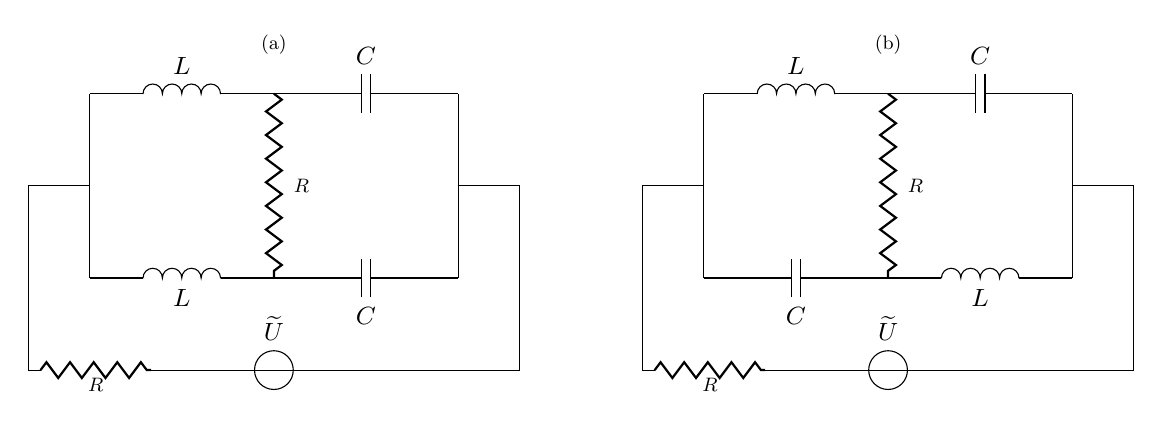
\begin{tikzpicture}[circuit ee IEC,scale=.78,transform shape,font=\small]
\begin{scope}[xshift=0cm]
\draw(-3,-1.5)--(-3,1.5);\draw(3,-1.5)--(3,1.5);
\draw(-3,1.5)to[inductor={info={$L$}}](0,1.5)to[capacitor={info={$C$}}](3,1.5);
\draw(-3,-1.5)to[inductor={info'={$L$}}](0,-1.5)to[capacitor={info'={$C$}}](3,-1.5);\draw[resistor](0,1.5)--(0,-1.5);\node[right,fill=white]at(.2,0){$R$};\draw(-3,0)--(-4,0)--(-4,-3)--(-3.8,-3);\draw[resistor](-3.8,-3)--(-2,-3)node[midway,below]{$R$};\draw(-2,-3)to[voltage source={info={$\widetilde U$}}](2,-3)--(4,-3)--(4,0)--(3,0);\node at(0,2.3){(a)};\end{scope}\begin{scope}[xshift=10cm]
\draw(-3,-1.5)--(-3,1.5);\draw(3,-1.5)--(3,1.5);
\draw(-3,1.5)to[inductor={info={$L$}}](0,1.5)to[capacitor={info={$C$}}](3,1.5);
\draw(-3,-1.5)to[capacitor={info'={$C$}}](0,-1.5)to[inductor={info'={$L$}}](3,-1.5);\draw[resistor](0,1.5)--(0,-1.5);\node[right,fill=white]at(.2,0){$R$};\draw(-3,0)--(-4,0)--(-4,-3)--(-3.8,-3);\draw[resistor](-3.8,-3)--(-2,-3)node[midway,below]{$R$};\draw(-2,-3)to[voltage source={info={$\widetilde U$}}](2,-3)--(4,-3)--(4,0)--(3,0);\node at(0,2.3){(b)};\end{scope}
\end{tikzpicture}

% 8 solution-04
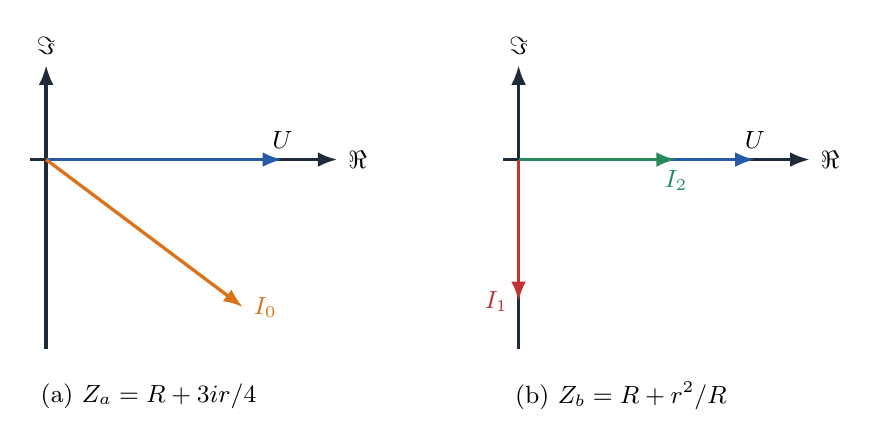
\begin{tikzpicture}[x=1cm,y=1cm,font=\small]

\begin{scope}[shift={(-4,0)}]\draw[axis](-.2,0)--(3.7,0)node[right]{$\Re$};\draw[axis](0,-2.4)--(0,1.2)node[above]{$\Im$};\draw[vec](0,0)--(3,0)node[above]{$U$};\draw[vec,orange](0,0)--(2.5,-1.875)node[right]{$I_0$};\node at(1.3,-3){(a) $Z_a=R+3ir/4$};\end{scope}
\begin{scope}[shift={(2,0)}]\draw[axis](-.2,0)--(3.7,0)node[right]{$\Re$};\draw[axis](0,-2.4)--(0,1.2)node[above]{$\Im$};\draw[vec](0,0)--(3,0)node[above]{$U$};\draw[vec,green](0,0)--(2,0)node[below]{$I_2$};\draw[vec,red](0,0)--(0,-1.8)node[left]{$I_1$};\node at(1.3,-3){(b) $Z_b=R+r^2/R$};\end{scope}
\end{tikzpicture}

% 9 question-05
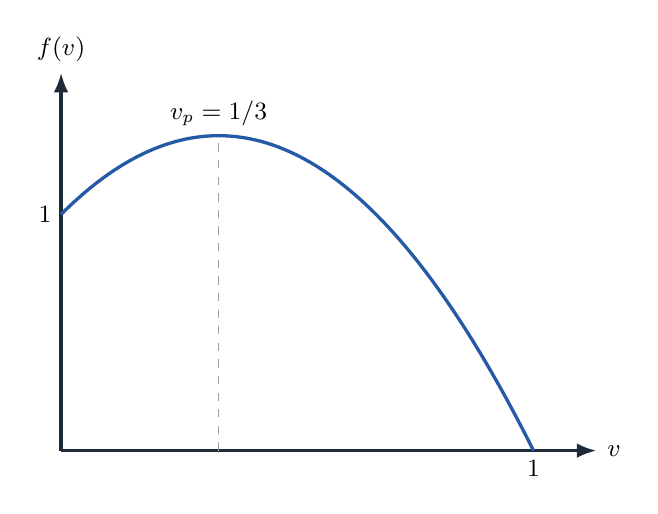
\begin{tikzpicture}[x=1cm,y=1cm,font=\small]
\draw[axis](0,0)--(6.8,0)node[right]{$v$};\draw[axis](0,0)--(0,4.8)node[above]{$f(v)$};\draw[very thick,blue] plot coordinates {(0.000000,3.000000) (0.043165,3.042700) (0.086331,3.084468) (0.129496,3.125304) (0.172662,3.165209) (0.215827,3.204182) (0.258993,3.242223) (0.302158,3.279333) (0.345324,3.315512) (0.388489,3.350758) (0.431655,3.385073) (0.474820,3.418457) (0.517986,3.450908) (0.561151,3.482428) (0.604317,3.513017) (0.647482,3.542674) (0.690647,3.571399) (0.733813,3.599193) (0.776978,3.626055) (0.820144,3.651985) (0.863309,3.676984) (0.906475,3.701051) (0.949640,3.724186) (0.992806,3.746390) (1.035971,3.767662) (1.079137,3.788003) (1.122302,3.807412) (1.165468,3.825889) (1.208633,3.843435) (1.251799,3.860049) (1.294964,3.875731) (1.338129,3.890482) (1.381295,3.904301) (1.424460,3.917189) (1.467626,3.929144) (1.510791,3.940169) (1.553957,3.950261) (1.597122,3.959422) (1.640288,3.967652) (1.683453,3.974950) (1.726619,3.981316) (1.769784,3.986750) (1.812950,3.991253) (1.856115,3.994824) (1.899281,3.997464) (1.942446,3.999172) (1.985612,3.999948) (2.028777,3.999793) (2.071942,3.998706) (2.115108,3.996688) (2.158273,3.993737) (2.201439,3.989856) (2.244604,3.985042) (2.287770,3.979297) (2.330935,3.972620) (2.374101,3.965012) (2.417266,3.956472) (2.460432,3.947001) (2.503597,3.936597) (2.546763,3.925263) (2.589928,3.912996) (2.633094,3.899798) (2.676259,3.885668) (2.719424,3.870607) (2.762590,3.854614) (2.805755,3.837690) (2.848921,3.819833) (2.892086,3.801045) (2.935252,3.781326) (2.978417,3.760675) (3.021583,3.739092) (3.064748,3.716578) (3.107914,3.693132) (3.151079,3.668754) (3.194245,3.643445) (3.237410,3.617204) (3.280576,3.590032) (3.323741,3.561927) (3.366906,3.532892) (3.410072,3.502924) (3.453237,3.472025) (3.496403,3.440195) (3.539568,3.407432) (3.582734,3.373738) (3.625899,3.339113) (3.669065,3.303556) (3.712230,3.267067) (3.755396,3.229646) (3.798561,3.191294) (3.841727,3.152011) (3.884892,3.111795) (3.928058,3.070649) (3.971223,3.028570) (4.014388,2.985560) (4.057554,2.941618) (4.100719,2.896744) (4.143885,2.850939) (4.187050,2.804203) (4.230216,2.756534) (4.273381,2.707934) (4.316547,2.658403) (4.359712,2.607940) (4.402878,2.556545) (4.446043,2.504218) (4.489209,2.450960) (4.532374,2.396770) (4.575540,2.341649) (4.618705,2.285596) (4.661871,2.228611) (4.705036,2.170695) (4.748201,2.111847) (4.791367,2.052068) (4.834532,1.991357) (4.877698,1.929714) (4.920863,1.867139) (4.964029,1.803633) (5.007194,1.739196) (5.050360,1.673826) (5.093525,1.607525) (5.136691,1.540293) (5.179856,1.472129) (5.223022,1.403033) (5.266187,1.333006) (5.309353,1.262046) (5.352518,1.190156) (5.395683,1.117333) (5.438849,1.043580) (5.482014,0.968894) (5.525180,0.893277) (5.568345,0.816728) (5.611511,0.739247) (5.654676,0.660835) (5.697842,0.581492) (5.741007,0.501216) (5.784173,0.420009) (5.827338,0.337871) (5.870504,0.254800) (5.913669,0.170799) (5.956835,0.085865) (6.000000,0.000000)};
\node[left]at(0,3){1};\node[below]at(6,0){1};\draw[guide](2,0)--(2,4)node[above]{$v_p=1/3$};
\end{tikzpicture}

% 10 solution-05
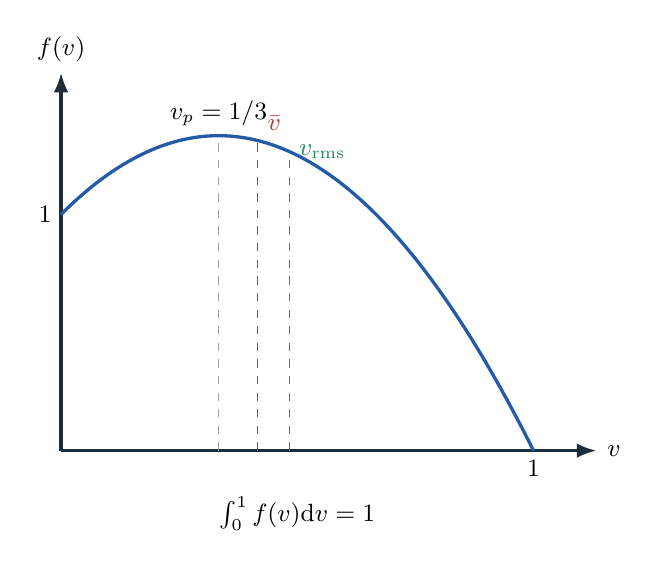
\begin{tikzpicture}[x=1cm,y=1cm,font=\small]
\draw[axis](0,0)--(6.8,0)node[right]{$v$};\draw[axis](0,0)--(0,4.8)node[above]{$f(v)$};\draw[very thick,blue] plot coordinates {(0.000000,3.000000) (0.043165,3.042700) (0.086331,3.084468) (0.129496,3.125304) (0.172662,3.165209) (0.215827,3.204182) (0.258993,3.242223) (0.302158,3.279333) (0.345324,3.315512) (0.388489,3.350758) (0.431655,3.385073) (0.474820,3.418457) (0.517986,3.450908) (0.561151,3.482428) (0.604317,3.513017) (0.647482,3.542674) (0.690647,3.571399) (0.733813,3.599193) (0.776978,3.626055) (0.820144,3.651985) (0.863309,3.676984) (0.906475,3.701051) (0.949640,3.724186) (0.992806,3.746390) (1.035971,3.767662) (1.079137,3.788003) (1.122302,3.807412) (1.165468,3.825889) (1.208633,3.843435) (1.251799,3.860049) (1.294964,3.875731) (1.338129,3.890482) (1.381295,3.904301) (1.424460,3.917189) (1.467626,3.929144) (1.510791,3.940169) (1.553957,3.950261) (1.597122,3.959422) (1.640288,3.967652) (1.683453,3.974950) (1.726619,3.981316) (1.769784,3.986750) (1.812950,3.991253) (1.856115,3.994824) (1.899281,3.997464) (1.942446,3.999172) (1.985612,3.999948) (2.028777,3.999793) (2.071942,3.998706) (2.115108,3.996688) (2.158273,3.993737) (2.201439,3.989856) (2.244604,3.985042) (2.287770,3.979297) (2.330935,3.972620) (2.374101,3.965012) (2.417266,3.956472) (2.460432,3.947001) (2.503597,3.936597) (2.546763,3.925263) (2.589928,3.912996) (2.633094,3.899798) (2.676259,3.885668) (2.719424,3.870607) (2.762590,3.854614) (2.805755,3.837690) (2.848921,3.819833) (2.892086,3.801045) (2.935252,3.781326) (2.978417,3.760675) (3.021583,3.739092) (3.064748,3.716578) (3.107914,3.693132) (3.151079,3.668754) (3.194245,3.643445) (3.237410,3.617204) (3.280576,3.590032) (3.323741,3.561927) (3.366906,3.532892) (3.410072,3.502924) (3.453237,3.472025) (3.496403,3.440195) (3.539568,3.407432) (3.582734,3.373738) (3.625899,3.339113) (3.669065,3.303556) (3.712230,3.267067) (3.755396,3.229646) (3.798561,3.191294) (3.841727,3.152011) (3.884892,3.111795) (3.928058,3.070649) (3.971223,3.028570) (4.014388,2.985560) (4.057554,2.941618) (4.100719,2.896744) (4.143885,2.850939) (4.187050,2.804203) (4.230216,2.756534) (4.273381,2.707934) (4.316547,2.658403) (4.359712,2.607940) (4.402878,2.556545) (4.446043,2.504218) (4.489209,2.450960) (4.532374,2.396770) (4.575540,2.341649) (4.618705,2.285596) (4.661871,2.228611) (4.705036,2.170695) (4.748201,2.111847) (4.791367,2.052068) (4.834532,1.991357) (4.877698,1.929714) (4.920863,1.867139) (4.964029,1.803633) (5.007194,1.739196) (5.050360,1.673826) (5.093525,1.607525) (5.136691,1.540293) (5.179856,1.472129) (5.223022,1.403033) (5.266187,1.333006) (5.309353,1.262046) (5.352518,1.190156) (5.395683,1.117333) (5.438849,1.043580) (5.482014,0.968894) (5.525180,0.893277) (5.568345,0.816728) (5.611511,0.739247) (5.654676,0.660835) (5.697842,0.581492) (5.741007,0.501216) (5.784173,0.420009) (5.827338,0.337871) (5.870504,0.254800) (5.913669,0.170799) (5.956835,0.085865) (6.000000,0.000000)};
\node[left]at(0,3){1};\node[below]at(6,0){1};\draw[guide](2,0)--(2,4)node[above]{$v_p=1/3$};\draw[red,dashed](2.5,0)--(2.5,3.9375)node[above right]{$\bar v$};\draw[green,dashed](2.898275,0)--(2.898275,3.798)node[right]{$v_{\rm rms}$};\node at(3,-.8){$\int_0^1f(v)\mathrm dv=1$};
\end{tikzpicture}

% 11 question-06
\begin{tikzpicture}[scale=1]
  \draw[body] (0,-2.3)--(0,2.3); \draw[body] (8,-2.3)--(8,2.3);
  \foreach \y in {-2,-1.5,...,2} {\draw[ink!50] (-.35,\y-.25)--(0,\y); \draw[ink!50] (8,\y)--(8.35,\y+.25);}
  \draw[vec] (3.0,.25)--(5.1,.25) node[midway,above] {光子 $\nu_0$};
  \draw[vec,red] (8,-.65)--(6.5,-.65) node[midway,below] {$u_0$};
  \draw[dim] (0,-3)--(8,-3) node[midway,below] {$l_0$};
  \node at (0,2.8) {固定镜}; \node at (8,2.8) {运动镜};
\end{tikzpicture}

% 12 solution-06
\begin{tikzpicture}[x=1cm,y=1cm,font=\small]
\draw[axis](0,0)--(3,0)node[right]{$X/l_0$};\draw[axis](0,0)--(0,7.2)node[above]{$ct/l_0$};\draw[very thick,orange] plot coordinates {(0.000000,0.000000) (0.000000,6.900000)};
\draw[very thick,red] plot coordinates {(2.000000,0.000000) (0.620000,6.900000)};
\draw[very thick,blue,-{Latex}] plot coordinates {(0.000000,0.000000) (1.818182,0.909091) (0.000000,1.818182) (1.487603,2.561983) (0.000000,3.305785) (1.217130,3.914350) (0.000000,4.522915) (0.995834,5.020832)};
\node[above]at(2,0){运动镜};\node[align=left,anchor=west]at(3.3,3.2){示例$u_0=0.1c$\\$X_{N+1}=X_N/q$\\$\nu_{N+1}=q\nu_N$\\同相位$\nu_NX_N$守恒};
\end{tikzpicture}

% 13 question-07
\begin{tikzpicture}[x=1cm,y=1cm,font=\small]

\fill[blue!7](-4,-1.7)rectangle(0,1.7);\draw[body](0,-1.7)--(0,1.7);\draw[body,fill=orange!12](0,-.9)..controls(.25,-.4)and(.25,.4)..(0,.9)--cycle;
\draw[axis](-4.5,0)--(3,0);\fill(-3,0)circle(2pt)node[below]{物点};\draw[dim](-3,-1.2)--(0,-1.2)node[midway,below]{$x$};
\node at(-2,1.4){水$4/3$};\node at(1.8,1.4){空气1};\node[align=left]at(1.9,-1.2){玻璃$3/2$\\曲率半径$R=f/2$};
\node at(-.7,-2.2){透镜厚度夸张示意；R是曲率半径};
\end{tikzpicture}

% 14 solution-07
\begin{tikzpicture}[scale=.8,font=\small]
\begin{scope}[shift={(0,0)}]\fill[blue!6](-6.4,-.9)rectangle(0,3.2);\draw[body](0,-.9)--(0,3.2);\draw[axis](-6.6,0)--(3.1,0);\draw[vec,orange](-2,0)--(-2,.7)node[above]{物};\draw[vec,red,dashed](-6,0)--(-6,2.8)node[above]{虚像};\draw[very thick,blue,-{Latex}] plot coordinates {(-2.000000,0.700000) (0.000000,0.700000) (2.800000,-0.280000)};
\draw[red,dashed] plot coordinates {(-6.000000,2.800000) (0.000000,0.700000)};
\draw[very thick,blue,-{Latex}] plot coordinates {(-2.000000,0.700000) (0.000000,1.200000) (2.800000,0.453333)};
\draw[red,dashed] plot coordinates {(-6.000000,2.800000) (0.000000,1.200000)};
\node at(-1.7,-1.6){外贴：$y=-3f,\beta=4$};\end{scope}\begin{scope}[shift={(10,0)}]\fill[blue!6](-6.4,-.9)rectangle(0,3.2);\draw[body](0,-.9)--(0,3.2);\draw[axis](-6.6,0)--(3.1,0);\draw[vec,orange](-2,0)--(-2,.7)node[above]{物};\draw[vec,red,dashed](-2,0)--(-2,0.9333333333333332)node[above]{虚像};\draw[very thick,blue,-{Latex}] plot coordinates {(-2.000000,0.700000) (0.000000,0.700000) (2.800000,0.373333)};
\draw[red,dashed] plot coordinates {(-2.000000,0.933333) (0.000000,0.700000)};
\draw[very thick,blue,-{Latex}] plot coordinates {(-2.000000,0.700000) (0.000000,1.200000) (2.800000,1.573333)};
\draw[red,dashed] plot coordinates {(-2.000000,0.933333) (0.000000,1.200000)};
\node at(-1.7,-1.6){内贴：$y\prime=-f,\beta\prime=4/3$};\end{scope}
\end{tikzpicture}

% 15 question-08
\begin{tikzpicture}[x=1cm,y=1cm,font=\small]

\draw[body,fill=blue!8](0,0)circle(1.8);\foreach\x/\y in{.6/.6,-.6/.6,.6/-.6,-.6/-.6,0/1.2,0/-1.2}{\node[blue]at(\x,\y){$\odot$};}
\draw[body,orange](-4,0)--(4,0);\node[mass]at(-4,0){$m$};\node[mass]at(4,0){$m$};\fill(0,0)circle(2pt)node[below]{转轴};
\draw[dim](-4,-2.4)--(4,-2.4)node[midway,below]{$L$};\draw[dim](0,2.4)--(1.8,2.4)node[midway,above]{$r$};
\draw[vec](2.8,0)--(2.8,1.1)node[right]{$E_\varphi$};\draw[vec](-2.8,0)--(-2.8,-1.1)node[left]{$E_\varphi$};
\node at(0,3.3){顶视图：$B_z>0,\dot B_z<0$};
\end{tikzpicture}

% 16 solution-08
\begin{tikzpicture}[x=1cm,y=1cm,font=\small]
\begin{scope}[shift={(-3.7,0)}]\draw[axis](0,0)--(4.7,0)node[right]{$x$};\draw[axis](0,0)--(0,2.6)node[above]{$2E_\varphi/(-\dot B)$};\draw[very thick,blue] plot coordinates {(0.000000,0.000000) (0.022346,0.022346) (0.044693,0.044693) (0.067039,0.067039) (0.089385,0.089385) (0.111732,0.111732) (0.134078,0.134078) (0.156425,0.156425) (0.178771,0.178771) (0.201117,0.201117) (0.223464,0.223464) (0.245810,0.245810) (0.268156,0.268156) (0.290503,0.290503) (0.312849,0.312849) (0.335196,0.335196) (0.357542,0.357542) (0.379888,0.379888) (0.402235,0.402235) (0.424581,0.424581) (0.446927,0.446927) (0.469274,0.469274) (0.491620,0.491620) (0.513966,0.513966) (0.536313,0.536313) (0.558659,0.558659) (0.581006,0.581006) (0.603352,0.603352) (0.625698,0.625698) (0.648045,0.648045) (0.670391,0.670391) (0.692737,0.692737) (0.715084,0.715084) (0.737430,0.737430) (0.759777,0.759777) (0.782123,0.782123) (0.804469,0.804469) (0.826816,0.826816) (0.849162,0.849162) (0.871508,0.871508) (0.893855,0.893855) (0.916201,0.916201) (0.938547,0.938547) (0.960894,0.960894) (0.983240,0.983240) (1.005587,1.005587) (1.027933,1.027933) (1.050279,1.050279) (1.072626,1.072626) (1.094972,1.094972) (1.117318,1.117318) (1.139665,1.139665) (1.162011,1.162011) (1.184358,1.184358) (1.206704,1.206704) (1.229050,1.229050) (1.251397,1.251397) (1.273743,1.273743) (1.296089,1.296089) (1.318436,1.318436) (1.340782,1.340782) (1.363128,1.363128) (1.385475,1.385475) (1.407821,1.407821) (1.430168,1.430168) (1.452514,1.452514) (1.474860,1.474860) (1.497207,1.497207) (1.519553,1.480699) (1.541899,1.459239) (1.564246,1.438393) (1.586592,1.418134) (1.608939,1.398438) (1.631285,1.379281) (1.653631,1.360642) (1.675978,1.342500) (1.698324,1.324836) (1.720670,1.307630) (1.743017,1.290865) (1.765363,1.274525) (1.787709,1.258594) (1.810056,1.243056) (1.832402,1.227896) (1.854749,1.213102) (1.877095,1.198661) (1.899441,1.184559) (1.921788,1.170785) (1.944134,1.157328) (1.966480,1.144176) (1.988827,1.131320) (2.011173,1.118750) (2.033520,1.106456) (2.055866,1.094429) (2.078212,1.082661) (2.100559,1.071144) (2.122905,1.059868) (2.145251,1.048828) (2.167598,1.038015) (2.189944,1.027423) (2.212291,1.017045) (2.234637,1.006875) (2.256983,0.996906) (2.279330,0.987132) (2.301676,0.977549) (2.324022,0.968149) (2.346369,0.958929) (2.368715,0.949882) (2.391061,0.941005) (2.413408,0.932292) (2.435754,0.923739) (2.458101,0.915341) (2.480447,0.907095) (2.502793,0.898996) (2.525140,0.891040) (2.547486,0.883224) (2.569832,0.875543) (2.592179,0.867996) (2.614525,0.860577) (2.636872,0.853284) (2.659218,0.846113) (2.681564,0.839062) (2.703911,0.832128) (2.726257,0.825307) (2.748603,0.818598) (2.770950,0.811996) (2.793296,0.805500) (2.815642,0.799107) (2.837989,0.792815) (2.860335,0.786621) (2.882682,0.780523) (2.905028,0.774519) (2.927374,0.768607) (2.949721,0.762784) (2.972067,0.757049) (2.994413,0.751399) (3.016760,0.745833) (3.039106,0.740349) (3.061453,0.734945) (3.083799,0.729620) (3.106145,0.724371) (3.128492,0.719196) (3.150838,0.714096) (3.173184,0.709067) (3.195531,0.704108) (3.217877,0.699219) (3.240223,0.694397) (3.262570,0.689640) (3.284916,0.684949) (3.307263,0.680321) (3.329609,0.675755) (3.351955,0.671250) (3.374302,0.666805) (3.396648,0.662418) (3.418994,0.658088) (3.441341,0.653815) (3.463687,0.649597) (3.486034,0.645433) (3.508380,0.641322) (3.530726,0.637263) (3.553073,0.633255) (3.575419,0.629297) (3.597765,0.625388) (3.620112,0.621528) (3.642458,0.617715) (3.664804,0.613948) (3.687151,0.610227) (3.709497,0.606551) (3.731844,0.602919) (3.754190,0.599330) (3.776536,0.595784) (3.798883,0.592279) (3.821229,0.588816) (3.843575,0.585392) (3.865922,0.582009) (3.888268,0.578664) (3.910615,0.575357) (3.932961,0.572088) (3.955307,0.568856) (3.977654,0.565660) (4.000000,0.562500)};
\draw[guide](1.5,0)--(1.5,1.5);\node[below]at(1.5,0){$r$};\node[below]at(4,0){$L/2$};\end{scope}\begin{scope}[shift={(2,0)}]\draw[axis](0,0)--(4.7,0)node[right]{$x$};\draw[axis](0,0)--(0,3.2)node[above]{力矩积分核};\draw[very thick,orange] plot coordinates {(0.000000,0.000000) (0.022346,0.000499) (0.044693,0.001997) (0.067039,0.004494) (0.089385,0.007990) (0.111732,0.012484) (0.134078,0.017977) (0.156425,0.024469) (0.178771,0.031959) (0.201117,0.040448) (0.223464,0.049936) (0.245810,0.060423) (0.268156,0.071908) (0.290503,0.084392) (0.312849,0.097875) (0.335196,0.112356) (0.357542,0.127836) (0.379888,0.144315) (0.402235,0.161793) (0.424581,0.180269) (0.446927,0.199744) (0.469274,0.220218) (0.491620,0.241690) (0.513966,0.264162) (0.536313,0.287631) (0.558659,0.312100) (0.581006,0.337567) (0.603352,0.364034) (0.625698,0.391498) (0.648045,0.419962) (0.670391,0.449424) (0.692737,0.479885) (0.715084,0.511345) (0.737430,0.543803) (0.759777,0.577260) (0.782123,0.611716) (0.804469,0.647171) (0.826816,0.683624) (0.849162,0.721076) (0.871508,0.759527) (0.893855,0.798976) (0.916201,0.839424) (0.938547,0.880871) (0.960894,0.923317) (0.983240,0.966761) (1.005587,1.011204) (1.027933,1.056646) (1.050279,1.103087) (1.072626,1.150526) (1.094972,1.198964) (1.117318,1.248400) (1.139665,1.298836) (1.162011,1.350270) (1.184358,1.402703) (1.206704,1.456134) (1.229050,1.510565) (1.251397,1.565994) (1.273743,1.622421) (1.296089,1.679848) (1.318436,1.738273) (1.340782,1.797697) (1.363128,1.858119) (1.385475,1.919541) (1.407821,1.981961) (1.430168,2.045379) (1.452514,2.109797) (1.474860,2.175213) (1.497207,2.241628) (1.519553,2.250000) (1.541899,2.250000) (1.564246,2.250000) (1.586592,2.250000) (1.608939,2.250000) (1.631285,2.250000) (1.653631,2.250000) (1.675978,2.250000) (1.698324,2.250000) (1.720670,2.250000) (1.743017,2.250000) (1.765363,2.250000) (1.787709,2.250000) (1.810056,2.250000) (1.832402,2.250000) (1.854749,2.250000) (1.877095,2.250000) (1.899441,2.250000) (1.921788,2.250000) (1.944134,2.250000) (1.966480,2.250000) (1.988827,2.250000) (2.011173,2.250000) (2.033520,2.250000) (2.055866,2.250000) (2.078212,2.250000) (2.100559,2.250000) (2.122905,2.250000) (2.145251,2.250000) (2.167598,2.250000) (2.189944,2.250000) (2.212291,2.250000) (2.234637,2.250000) (2.256983,2.250000) (2.279330,2.250000) (2.301676,2.250000) (2.324022,2.250000) (2.346369,2.250000) (2.368715,2.250000) (2.391061,2.250000) (2.413408,2.250000) (2.435754,2.250000) (2.458101,2.250000) (2.480447,2.250000) (2.502793,2.250000) (2.525140,2.250000) (2.547486,2.250000) (2.569832,2.250000) (2.592179,2.250000) (2.614525,2.250000) (2.636872,2.250000) (2.659218,2.250000) (2.681564,2.250000) (2.703911,2.250000) (2.726257,2.250000) (2.748603,2.250000) (2.770950,2.250000) (2.793296,2.250000) (2.815642,2.250000) (2.837989,2.250000) (2.860335,2.250000) (2.882682,2.250000) (2.905028,2.250000) (2.927374,2.250000) (2.949721,2.250000) (2.972067,2.250000) (2.994413,2.250000) (3.016760,2.250000) (3.039106,2.250000) (3.061453,2.250000) (3.083799,2.250000) (3.106145,2.250000) (3.128492,2.250000) (3.150838,2.250000) (3.173184,2.250000) (3.195531,2.250000) (3.217877,2.250000) (3.240223,2.250000) (3.262570,2.250000) (3.284916,2.250000) (3.307263,2.250000) (3.329609,2.250000) (3.351955,2.250000) (3.374302,2.250000) (3.396648,2.250000) (3.418994,2.250000) (3.441341,2.250000) (3.463687,2.250000) (3.486034,2.250000) (3.508380,2.250000) (3.530726,2.250000) (3.553073,2.250000) (3.575419,2.250000) (3.597765,2.250000) (3.620112,2.250000) (3.642458,2.250000) (3.664804,2.250000) (3.687151,2.250000) (3.709497,2.250000) (3.731844,2.250000) (3.754190,2.250000) (3.776536,2.250000) (3.798883,2.250000) (3.821229,2.250000) (3.843575,2.250000) (3.865922,2.250000) (3.888268,2.250000) (3.910615,2.250000) (3.932961,2.250000) (3.955307,2.250000) (3.977654,2.250000) (4.000000,2.250000)};
\draw[guide](1.5,0)--(1.5,2.25);\node[below]at(1.5,0){$r$};\node[below]at(4,0){$L/2$};\node at(2,-1){$x^2$内区，$r^2$外区};\end{scope}
\end{tikzpicture}
\end{document}
